% paper # 3887, pw CF8FECE1
% Note: the original submission was rev. 530... 
% submitted again at 539 before review..
% Template for SLT-2006 paper; to be used with:
%          spconf.sty  - ICASSP/ICIP LaTeX style file, and
%          IEEEbib.bst - IEEE bibliography style file.
% --------------------------------------------------------------------------
\documentclass{article}
\usepackage{spconf,amsmath,amssymb,bm,epsfig}
\usepackage{color}
\usepackage{multirow}

\definecolor{MidGray}{rgb}{0.3, 0.3, 0.3}
\definecolor{Pink}{rgb}{1.0, 0.4, 0.4}
\definecolor{Red}{rgb}{0.9, 0.1, 0.1}

% Example definitions.
% --------------------

%%%%%%
% Begin Dan's math definitions.
%%%%%%
\def\Re{{\mathbb{R}}}
\def\x{{\mathbf x}}
\def\a{{\mathbf a}}
\def\U{{\mathbf U}}
\def\HCLG{{\mathit{HCLG}}}
\def\bDelta{{\mathbf \Delta}}
\def\V{{\mathbf V}}
\def\u{{\mathbf u}}
\def\s{{\mathbf s}}
\def\t{{\mathbf t}}
\def\G{{\mathbf G}}
\def\F{{\mathbf F}}
\def\r{{\mathbf r}}
\def\semicolonsep{\,;\,}
\def\tr{{\operatorname{tr}\,}}
\def\z{{\mathbf z}}
\def\y{{\mathbf y}}
\def\Y{{\mathbf Y}}
\def\Z{{\mathbf Z}}
\def\gammatilde{{\gamma}}  %% This was \tilde{\gamma} in the tutorial, mapping to \gamma2 to preserve the distinction in the latex source in case later I want to resurrect that.
\def\R{{\mathbf R}}
\def\D{{\mathbf D}}
\def\half{ {\textstyle {\frac{1}{2}}} }
\def\L{{\mathbf L}}
\def\P{{\mathbf P}}
\def\Q{{\mathbf Q}}
\def\B{{\mathbf B}}
\def\S{{\mathbf S}}
\def\T{{\mathbf T}}
\def\K{{\mathbf K}}
\def\H{{\mathbf H}}
\def\g{{\mathbf g}}
\def\I{{\mathbf I}}
\def\btheta{{\mathbf\theta}}
\def\calN{{\cal N}}
\def\calQ{{\cal Q}}
\def\diag{{\mathrm{diag}}}
\def\pre{{\mathrm{pre}}}
\def\inv{{\mathrm{inv}}}
\def\calT{{\cal T}}
\def\bmu{{\bm \mu}} % mathbf does not work for lowercase greek letters!  But mathbf looks better than bm in most other cases so I only use bm here.
\def\bSigma{{\mathbf \Sigma}}
\def\M{{\mathbf M}}
\def\N{{\mathbf N}}
\def\bv{{\mathbf v}}
\def\w{{\mathbf w}}
\def\W{{\mathbf W}}
\def\A{{\mathbf A}}
\def\o{{\mathbf o}}
\def\b{{\mathbf b}}
\def\p{{\mathbf p}}
%%\newcommand\refeqn[1]{(\ref{#1})}

%%%%%%
% End Dan's math definitions.
%%%%%%


% Title.
% ------
\title{Generating exact lattices in the WFST framework}


\makeatletter
\def\name#1{\gdef\@name{#1\\}}
\makeatother

\name{ \em Daniel Povey$^1$, Mirko Hannemann$^{1,2}$,  \\
 \em {Gilles Boulianne}$^3$, {Luk\'{a}\v{s} Burget}$^{2,4}$, {Arnab Ghoshal}$^5$, {Milo\v{s} Janda}$^2$, {Martin Karafi\'{a}t}$^2$, {Stefan Kombrink}$^2$, \\
  \em {Petr Motl\'{i}\v{c}ek}$^6$, {Yanmin Qian}$^7$, {Korbinian Riedhammer}$^9$, {Karel Vesel\'{y}}$^2$, {Ngoc Thang Vu}$^8$
    \thanks{Thanks to Honza \v{C}ernock\'{y}, Renata Kohlov\'{a}, and Tom\'{a}\v{s} Ka\v{s}p\'{a}rek for their help relating to the Kaldi'11 workshop at BUT, and to Sanjeev Khudanpur for his help in preparing the paper.  Researchers at BUT were partly supported by Technology Agency of the Czech Republic grant No. TA01011328, Czech Ministry of Education project No. MSM0021630528, and Grant Agency of the Czech Republic project No. 102/08/0707.  Arnab Ghoshal was supported by EC FP7 grant 213850 (SCALE), and by EPSRC grant EP/I031022/1 (NST).}}


%%% TODO: fix thanks.
%\thanks{Arnab Ghoshal was supported by the European Community's Seventh Framework 
% Programme under grant agreement no. 213850 (SCALE); BUT researchers were partially 
%supported by Czech MPO project No. FR-TI1/034.}}
       
\address{{ $^1$ Microsoft Research, Redmond, WA, {\normalsize \tt dpovey@microsoft.com} }\\ 
         { $^2$ Brno University of Technology, Czech Republic, {\normalsize \tt ihannema@fit.vutbr.cz}} \\ 
         { $^3$ CRIM, Montreal, Canada \ \  $^4$ SRI International, Menlo Park, CA, USA} \\ 
         { $^5$ University of Edinburgh, U.K. \ \  $^6$  IDIAP, Martigny, Switzerland } \\ 
         { $^7$ Tsinghua University, Beijing, China \ \ $^8$ Karlsruhe Institute of Technology, Germany} \\ 
         { $^9$ Pattern Recognition Lab, University of Erlangen-Nuremberg, Germany}}

 
\begin{document}


\ninept  
%
\maketitle
%
%\pagestyle{plain} % was set to empty in spconf.sty... this makes page number appear.

\begin{abstract}
We describe a lattice generation method that is exact, i.e. it satisfies all the 
natural properties we would want from a lattice of alternative transcriptions of
an utterance.  This method does not introduce substantial overhead above one-best decoding.  Our method is
most directly applicable when using WFST decoders where the WFST is
``fully expanded'', i.e. where the arcs correspond to HMM transitions.  It outputs
lattices that include HMM-state-level alignments as well as word labels.
The general idea is to create a state-level lattice during decoding, and to do
a special form of determinization that retains only the best-scoring path
for each word sequence.  
This special determinization algorithm is a solution to the following problem:
Given a WFST A, compute a WFST B that, for each input-symbol-sequence of A,
contains just the lowest-cost path through A.
\end{abstract}

\begin{keywords}
  Speech Recognition, Lattice Generation
\end{keywords}

\vspace*{-0.075in}
\section{Introduction}
\vspace*{-0.05in}

In Section~\ref{sec:wfst} we give a Weighted Finite State Transducer
(WFST) interpretation of the speech-recognition decoding problem, in order
to introduce notation for the rest of the paper.  In Section~\ref{sec:lattices}
we define the lattice generation problem, and in Section~\ref{sec:previous}
we review previous work.
In Section~\ref{sec:overview} we give an overview of our method,
and in Section~\ref{sec:details} we summarize some aspects of a determinization
algorithm that we use in our method.  In Section~\ref{sec:exp} we give
experimental results, and in Section~\ref{sec:conc} we conclude.

\vspace*{-0.075in}
\section{WFSTs and the decoding problem}
\vspace*{-0.05in}
\label{sec:wfst}

The graph creation process we use in our toolkit, Kaldi~\cite{kaldi_paper},
is very close to the standard recipe described in~\cite{wfst},
where the Weighted Finite State Transducer (WFST) decoding graph is
\begin{equation}
  \HCLG = \min(\det(H \circ C \circ L \circ G)),
\end{equation}
where $H$, $C$, $L$ and $G$ represent the HMM structure, phonetic
context-dependency, lexicon and grammar respectively, 
and $\circ$ is WFST composition (note: view $\HCLG$ as a single symbol).
For concreteness we will speak of ``costs'' rather
than weights, where a cost is a floating point number that typically represents a negated
log-probability.  A WFST has a set of states with one distinguished
start state\footnote{This is the formulation that corresponds best with the toolkit we use.};
each state has a final-cost (or $\infty$ for non-final states);
and there is a set of arcs between the states, where each arc has an
input label, an output label, and a weight
(just think of this as a cost for now).
In $\HCLG$, the input labels are the identifiers of context-dependent
HMM states, and the output labels represent words.  For both the input and output
labels, the special symbol $\epsilon$ may appear, meaning ``no label is present.''


\begin{figure}
\begin{center}
\includegraphics[height=2.1in,angle=270]{figures/acceptor_utterance.eps}
\vspace*{-0.03in}
  \caption{Acceptor $U$ describing the acoustic scores of an utterance}
\vspace*{-0.15in}
\label{fig:acceptor}
\end{center}

\end{figure}

Imagine we want to ``decode'' an utterance of $T$ frames, i.e. we want to
find the most likely word sequence and its corresponding state-level alignment.  A WFST
interpretation of the decoding problem is as follows.  We construct an
acceptor, or WFSA, as in Fig.~\ref{fig:acceptor} (an acceptor is represented as a
WFST with identical input and output symbols).  It has $T{+}1$ states,
with an arc for each combination of (time, context-dependent HMM state).  The
costs on these arcs correspond to negated and scaled acoustic log-likelihoods.
Call this acceptor $U$.  Define
\begin{equation}
   S \equiv U \circ \HCLG,
\end{equation}
which we call the {\em search graph} of the utterance.  It has approximately $T{+}1$ times
more states than $\HCLG$ itself.  The decoding problem is equivalent to finding
the best path through $S$.  The input symbol sequence for this best path represents
the state-level alignment, and the output symbol sequence is the corresponding
sentence.  In practice we do not do a full search of $S$, but use beam pruning.
Let $B$ be the searched subset of $S$, containing a subset of the states and arcs
of $S$ obtained by some heuristic pruning procedure.  
When we do Viterbi decoding with beam-pruning, we are finding the best path through $B$. 
%
Since the beam pruning is a part of any practical search procedure and cannot
easily be avoided, we will define the desired outcome of lattice generation in terms
of the visited subset $B$ of $S$.

\vspace*{-0.075in}
\section{The lattice generation problem}
\vspace*{-0.05in}
\label{sec:lattices}


There is no generally accepted single definition of a lattice.  In~\cite{efficient_general}
and~\cite{sak2010fly}, it is defined as a labeled, weighted, directed acyclic graph
(i.e. a WFSA, with word labels).  In~\cite{ney_word_graph}, time information
is also included.  In the HTK lattice format~\cite{htkbook}, phone-level time alignments 
are also supported (along with separate language model, acoustic and pronunciation-probability 
scores), and in~\cite{saon2005anatomy}, HMM-state-level alignments are also produced.
In our work here we will be producing state-level alignments; in fact, the input-symbols
on our graph, which we call {\em transition-ids}, are slightly more fine-grained
than acoustic states and contain sufficient information to reconstruct the phone
sequence.  

There is, as far as we know, no generally accepted problem statement
for lattice generation, but all the the authors we cited seem to
be concerned with the accuracy of the information in the lattice (e.g. that the
scores and alignments are correct) and the completeness of such information (e.g.
that no high-scoring word-sequences are missing).  The simplest
way to formalize these concerns is to express them in terms of a lattice 
pruning beam $\alpha > 0$ (interpret this as a log likelihood difference).
\begin{itemize}
  \item The lattice should have a path for every word sequence within $\alpha$ of the best-scoring one.
  \item The scores and alignments in the lattice should be accurate.
  \item The lattice should not contain duplicate paths with the same word sequence.
\end{itemize}
We need to be a little more precise about what we mean by the scores
and alignments being ``accurate''.  Let the lattice be $L$.  The 
way we would like to state this requirement is:
\begin{itemize}
  \item For every path in $L$, the score and alignment corresponds to 
   the best-scoring path in $B$ for the corresponding word
   sequence\footnote{Or one of the best-scoring paths, in case of a tie.}.
\end{itemize}
The way we actually have to state the requirement in order to get an efficient procedure is:
\begin{itemize}
  \item For every word-sequence in $B$ within $\alpha$ of the best one, the score and alignment
    for the corresponding path in $L$ is accurate.
  \item All scores and alignments in $L$ correspond to actual paths through $B$ (but not always
   necessarily the best ones).
\end{itemize}
The issue is that we want to be able to prune $B$ before generating a lattice from it,
but doing so could cause paths not within $\alpha$ of the best one to be lost, so we have
to weaken the condition.  This is no great loss, since regardless
of pruning, any word-sequence not within $\alpha$ of the best one could be omitted altogether, 
which is the same as being assigned a cost of $\infty$).
By ``word-sequence'' we mean a sequence of whatever symbols are on the
output of $\HCLG$.  In our experiments these output symbols represent words, but
silences do not appear as output symbols (they are
represented via alternative paths in $L$).

\vspace*{-0.075in}
\section{Previous lattice generation methods}
\vspace*{-0.05in}
\label{sec:previous}

Lattice generation algorithms tend to be closely linked to particular types of decoder,
but are often justified by the same kinds of ideas.
A common assumption underlying lattice generation methods is the {\em word-pair assumption}
of~\cite{ney_word_graph}.  This is the notion that the time boundary between a pair of words
is not affected by the identity of any earlier words.  In a decoder in which there is
a different copy of the lexical tree for each preceding word, 
assuming the word-pair assumption holds, in order to generate an accurate lattice, it is
sufficient to store a single Viterbi back-pointer at the word level; the entire set of
such back-pointers contains enough information to generate the lattice.  Authors who have used
this type of lattice generation method~\cite{ney_word_graph,odell_thesis} have generally
not been able to evaluate how correct the word-pair assumption is in practice, but it seems
unlikely to cause problems.  Such methods are not applicable for WFST based decoders anyway.

The lattice generation method described in~\cite{efficient_general} 
is applicable to decoders that use WFSTs~\cite{wfst}
expanded down to the $C$ level (i.e. $CLG$), so the input symbols represent
context-dependent phones.  In WFST based decoding networks, states normally do
not have a unique one-word history, but the authors of~\cite{efficient_general}
were able to satisfy a similar condition at the phone level.  Their method was
to store a single Viterbi back-pointer at the phone level; use this to 
create a phone-level latice; prune the resulting
lattice; project it to leave only word labels; and then remove $\epsilon$
symbols and determinize.
Note that the form of pruning referred to here is not the same as beam pruning as
it takes account of both the forward and backward parts of the cost.
The paper also reported experiments with an accurate, ``reference'' method that did not require any
phone-pair assumption; these experiments showed that the main method they were describing
had almost the same lattice oracle error rate as the reference method.  However, the 
experiments did not evaluate how much impact the assumption had on the accuracy of the scores, 
and this information could be important in some applications.

The lattice generation algorithm that was described in~\cite{saon2005anatomy}
is applicable to WFSTs expanded down to the $H$ level (i.e. $\HCLG$),
so the input symbols represent context-dependent states.  It keeps both scores and 
state-level alignment information.  In some sense this algorithm also relies
on the word-pair assumption, but since the copies of the lexical tree in the decoding
graph do not have unique word histories, the resulting algorithm has to be quite
different.  Viterbi back-pointers at the word level are used, but the algorithm keeps track
of not just a single back-pointer in each state, but the $N$ best back-pointers for the $N$ top-scoring distinct
word histories.  Therefore, this algorithm has more in common with the sentence N-best
algorithm than with the Viterbi algorithm.  By limiting $N$ to be quite small (e.g. $N{=}5$),
the algorithm was made efficient, but at the cost of losing word sequences
that would be within the lattice-generation beam.

\vspace*{-0.075in}
\section{Overview of our algorithm}
\vspace*{-0.05in}
\label{sec:overview}

\subsection{Version without alignments}
\vspace*{-0.05in}

In order to explain our algorithm in the easiest way, we will first explain how it would
be if we did not keep the alignment information, and were storing only a single cost
(i.e. the total acoustic plus language-model cost).  This is just for didactic purposes;
we have not implemented this simple version.
In this case, our algorithm would be quite similar
to~\cite{efficient_general}, except at the state level rather than the phone level.
We actually store forward rather than backward pointers: for each active state on each
frame, we create a forward link record for each active arc out of that state; this points
to the record for the destination state of the arc on the next frame (or on 
the current frame, for $\epsilon$-input
arcs).   As in~\cite{efficient_general}, at the end of the utterance,
we prune the resulting graph to discard any paths that are not within the beam $\alpha$ of the best cost. 
Let the pruned graph be $P$, i.e.
\begin{equation}
  P = \mathrm{prune}(B, \alpha),
\end{equation}
where $B$ is the un-pruned state-level lattice.
We project on the output labels (i.e. we keep only the word labels), then remove $\epsilon$
arcs and determinize.  In fact, we use a determinization algorithm that does $\epsilon$
removal itself.

As in~\cite{efficient_general}, to save memory, we actually do the pruning
periodically rather than waiting for the end of the file (we do it every 25 frames).
Our method is equivalent to their method of linking all currently active states to a ``dummy''
final state and then pruning in the normal way.  However, we implement it in such a way
that the pruning algorithm does not always have to go back to the beginning of the utterance.
For each still-active state, we store the cost difference between the best path including that
state, and the best overall path.  This quantity does not always change between different
iterations of calling the pruning algorithm, and when we detect that these quantities are 
unchanged for a particular frame, the pruning algorithm can stop going backward in time.

After the determinization phase, we prune again using the beam $\alpha$.  This is needed because
the determinization process can introduce a lot of unlikely arcs.  In fact, for particular
utterances, the determinization process can cause the lattice to expand enough to
exhaust memory.  To deal with this, we currently just detect when determinization
has produced more than a pre-set maximum number of states, then we prune with a tighter
beam and try again.

This ``simple'' version of the algorithm produces an acyclic, deterministic
WFSA with words as labels.  This is sufficient for applications such as language-model
rescoring.

\vspace*{-0.075in}
\subsection{Keeping separate graph and acoustic costs}
\vspace*{-0.05in}

A fairly trivial extension of the algorithm described above is to store separately
the acoustic costs and the costs arising from $\HCLG$.  This enables us to do things
like generating output from the lattice with different acoustic scaling factors.
We refer to these two costs as the graph cost and the acoustic cost, since the cost
in $\HCLG$ is not just the language model cost but also contains components
arising from transition probabilities and pronunciation probabilities.  We implement
this by using a semiring that contains two real numbers, one for the graph and one
for the acoustic costs; it keeps track of the two costs separately, but its
$\oplus$ operation returns whichever pair has the lowest sum of costs (graph plus acoustic).

Formally, if each weight is a pair $(a,b)$, then $(a,b) \otimes (c,d) = (a{+}c, b{+}d)$,
and $(a,b) \oplus (c,d)$ is equal to $(a,b)$ if $a{+}b < c{+}d$ or if $a{+}b = c{+}d$ and $a{-}b < c{-}d$,
and otherwise is equal to $(c,d)$.  This is equivalent to the normal lexicographic semiring (see~\cite{roark2011lexicographic}) on the pair $((a{+}b),(a{-}b))$.

\vspace*{-0.075in}
\subsection{Keeping state-level alignments}
\vspace*{-0.05in}

It is useful for various purposes, e.g. discriminative training and certain kinds of
acoustic rescoring, to keep the state-level alignments in the lattices.  We will now
explain how we can make the alignments ``piggyback'' on top of the computation
defined above, by encoding them in a special semiring.

First, let us define $Q = \inv(P)$, i.e. $Q$ is the inverted, pruned state-level lattice,
where the input symbols are the words and the output symbols are the p.d.f. labels.
We want to process $Q$ in such a way that we keep only the best path through it
for each word sequence, and get the corresponding alignment.  This is possible
by defining an appropriate semiring and then doing normal determinization.  We shall
ignore the fact that we are keeping track of separate graph and acoustic costs, 
to avoid complicating the present discussion.  

We will define a semiring in which symbol sequences are encoded into the weights.
Let a weight be a pair $(c, s)$, where $c$ is a cost and $s$ is a sequence of symbols.
We define the $\otimes$ operation as $(c, s) \otimes (c', s') = (c+c', (s,s'))$, where
$(s,s')$ is a concatenation of $s$ and $s'$.  We define the $\oplus$ operation so that
it returns whichever pair has the smallest cost: that is, $(c,s) \oplus (c',s')$ 
equals $(c,s)$ if $c < c'$, and $(c',s')$ if $c > c'$.  If the costs are identical,
we cannot arbitrarily return the first pair because this would not satisfy the semiring
axioms.  In this case, we return the pair with the shorter string part, and if
the lengths are the same, whichever string appears first in dictionary order. 

Let $E$ be an encoding of the inverted state-level lattice $Q$ 
as described above, with the same number of states and arcs; $E$ is an acceptor, with its symbols
equal to the input symbol (word) on the corresponding arc of $Q$, and
the weights on the arcs of $E$ containing both the weight and the output symbol (p.d.f.),
if any, on the corresponding arcs of $Q$.  Let $D = \mathrm{det}(\mathrm{rmeps}(E))$.
Determinization
will always succeed because $E$ is acyclic (as long as the original decoding
graph $\HCLG$ has no $\epsilon$-input cycles).  Because $D$ is deterministic
and $\epsilon$-free, it has only one path for each word sequence. 
Determinization preserves equivalence,
and equivalence is defined in such a way that the $\oplus$-sum of the
weights of all the paths through $E$ with a particular word-sequence, must be the same
as the weight of the corresponding path through $D$ with that word-sequence.
It is clear from the definition of $\oplus$ that this path through
$D$ has the cost and alignment of the lowest-cost path through $E$ that has the
same word-sequence on it.  

\vspace*{-0.075in}
\subsection{Summary of our algorithm}
\vspace*{-0.05in}

During decoding, we create a data-structure
corresponding to a full state-level lattice.  That is, for every arc of $\HCLG$, we traverse
on every frame, we create a separate arc in the state-level lattice.  These arcs
contain the acoustic and graph costs separately.  We prune the state-level graph using
a beam $\alpha$; we do this periodically (every 25 frames) but this is equivalent to
doing it just once at the end, as in~\cite{efficient_general}.  Let the 
final pruned state-level lattice be $P$.
Let $Q = \inv(P)$, and let $E$ be an encoded version of $Q$ as described above (with the
state labels as part of the weights).  The final lattice is
\vspace*{-0.075in}
\begin{equation}
   L = \mathrm{prune}(\mathrm{det}(\mathrm{rmeps}(E)), \alpha) . \vspace*{-0.075in}
\end{equation}
The determinization and epsilon removal are done together by a single algorithm
that we will describe below.  $L$ is a deterministic, acyclic weighted acceptor with the 
words as the labels, and the graph and acoustic costs and the alignments
encoded into the weights.  The costs and alignments are not ``synchronized'' 
with the words.

\vspace*{-0.075in}
\section{Details of our determinization algorithm}
\vspace*{-0.05in}
\label{sec:details}

We implemented $\epsilon$ removal and determinization as a single algorithm 
because $\epsilon$-removal using the traditional approach would greatly
increase the size of the state-level lattice (this is mentioned 
in~\cite{efficient_general}).  Our algorithm uses data-structures
specialized for the particular type of weight we are using.  The issue
is that the determinization process often has to append a single symbol to
a string of symbols, and the easiest way to
do this in ``generic'' code would involve copying the whole sequence each time.
Instead we use a data structure that enables this to be done in linear
time (it involves a hash table).  

We will briefly describe another unique aspect of our
algorithm.  Determinization algorithms involve weighted subsets of states, e.g.:
\begin{equation}
   S = \{ (s_1, w_1), (s_2, w_2), \ldots \} .
\end{equation}
Let this weighted subset, as it appears in a conventional determinization
algorithm with epsilon removal, be the {\em canonical representation} of a state.
A typical determinization algorithm would maintain a map from this representation
to a state index.  We define a {\em minimial representation} of a state
to be like the canonical representation, but only keeping states that
are either final, or have non-$\epsilon$ arcs out of them.  We maintain
a map from the minimal representation to the state index.  We can
show that this algorithm is still correct (it will tend to give more
minimal output).   As an optimization for speed, we also define
the {\em initial representation} to be the same type of subset, but prior
to following through the $\epsilon$ arcs, i.e. it only contains the states
that we reached by following non-$\epsilon$ arcs from a previous determinized
state.  We maintain a separate map from the initial representation to
the output state index; think of this as a ``lookaside buffer'' that helps us
avoid the expense of following $\epsilon$ arcs. 

%Although we have not written a proof of correctness of this algorithm, we
%have tested it thoroughly.  This is done by generating random WFSTS,
%applying this algorithm, and if it terminates, checking that the result
%is deterministic and is equivalent (in this semiring) to the original WFST
%represented as an acceptor in this semiring.

Since submitting this paper, we have become aware of~\cite{shafran2011efficient},
which solves the exact same problem for a different purpose.  They use a semiring
which is more complicated than ours (the string part of the semiring becomes a
structured object with parentheses).  They use this semiring instead of the one
 we describe here, because in our semiring the $\oplus$-sum of two weights 
does not necessarily left-divide the weights, and this is a problem for 
a typical determinization algorithm.  We bypass
this problem by defining a ``common divisor'' operation $\boxplus$ with the
right properties (it $\oplus$-adds the weight part and returns the longest
common prefix of the string part).  We use this instead of
$\oplus$ when finding divisors in the determinization algorithm.


%% The algorithm for $\epsilon$-removal and determinization is also optimized
%% for our particular case.  We will first explain what a generic $\epsilon$-removal
%% and determinization algorithm would look like.  We will explain this using
%% generic weights.  Let us use the notation
%% \begin{equation}
%%    S = \{ (s_1, w_1), (s_2, w_2), \ldots \}
%% \end{equation}
%% for a weighted subset of states in the original FST.  Each subset $S$ corresponds
%% to a state in the determinized FST, i.e. we maintain a map $m(S) \rightarrow s$
%% where $s$ is a state number in the output (in practice there are tolerances
%% involved in this map when the weights contain floating-point numbers).  We need
%% to normalize these subsets to remove any ``common part'' of the weights.  We
%% need to define an associative and commutative ``common divisor'' operation 
%% on weights (call this $\boxplus$; it can be the same as $\oplus$ for many semirings),
%% that gives us the normalizer for a pair of weights.
%% We must be able to  left-divide each individual weight by the result of this operation, i.e.
%% if $c = a \boxplus b$, then we need to be able to solve $a = c a'$ and $b = c b'$ for $a'$ and $b'$.
%% Here, $a'$ and $b'$ become the ``normalized weights''.  Also $\otimes$-multiplication
%% must be left-distributive over this operation, which ensures the right kind of
%% ``uniqueness'' of the normalization operation.  In the particular case of interest
%% $w$ is a pair $(w', s)$ of a ``base-weight'' and a string $s$, and the 
%% operation $(a,s) \boxplus (b,t)$ returns $(a\oplus b, u)$ where $u$ is the longest
%% common prefix of $s$ and $t$ and $a\oplus b$ essentially returns the minimum cost.

%% For the determinization algorithm, we define
%% $\mathrm{normalizer}(S)$ to be the $\boxplus$-sum of the weights in the subset $S$,
%% and $\mathrm{normalize}(S)$ to be $S$ with each weight left-divided by 
%% $\mathrm{normalizer}(S)$.  We also need to define an operation that ``follows through''
%% $\epsilon$ transitions.  Call this $\mathrm{follow-eps}(S)$ 




%% The key characteristic of our method is that unlike all previously reported 
%% methods that we are aware of (with the sole exception of the inefficient method used 
%% as a baseline in~\cite{efficient_general}), our method is exact even if the word-pair 
%% assumption is invalid.  In addition, we are able to generate a lattice with full
%% state-level alignment information, which would not be possible using the approaches
%% used in~\cite{efficient_general}.  Our algorithm also does not need to store $N$
%% back-pointers like the lattice-generation algorithm previously reported in~\cite{saon2005anatomy}
%% for $H$-level WFSTs (i.e. fully-expanded WFSTs).  


\vspace*{-0.1in}
\section{Experimental results}
\vspace*{-0.075in}
\label{sec:exp}


We do not compare with any other algorithms,
as~\cite{ney_word_graph,odell_thesis,efficient_general} are designed for
different types of decoders than ours, and the lattices contain less information,
making comparisons hard to interpret; the algorithm of~\cite{saon2005anatomy} has
similar requirements and outputs as ours, but besides being inexact, it is bound
to be slower due to the need to store $N$ back-pointers, so we did not view it as
worthwhile to do the experiment.

We report experimental results on the Wall Street Journal database of
read speech. 
Our system is a standard mixture-of-Gaussians system trained on the SI-284
training data; we test on the November 1992 evaluation data.  
We generated lattices with the bigram language model
supplied with the WSJ database, and for rescoring experiments we
use the trigram language model.  The acoustic scale was $1/16$ for first-pass
decoding and $1/15$ for LM rescoring.  
For simplicity, we used a decoder that
does not support a ``maximum active states'' option, so the only variables
to consider are the beam used in the Viterbi beam search, and the separate
beam $\alpha$ used for lattice generation.

\begin{figure}[t]
\centering
   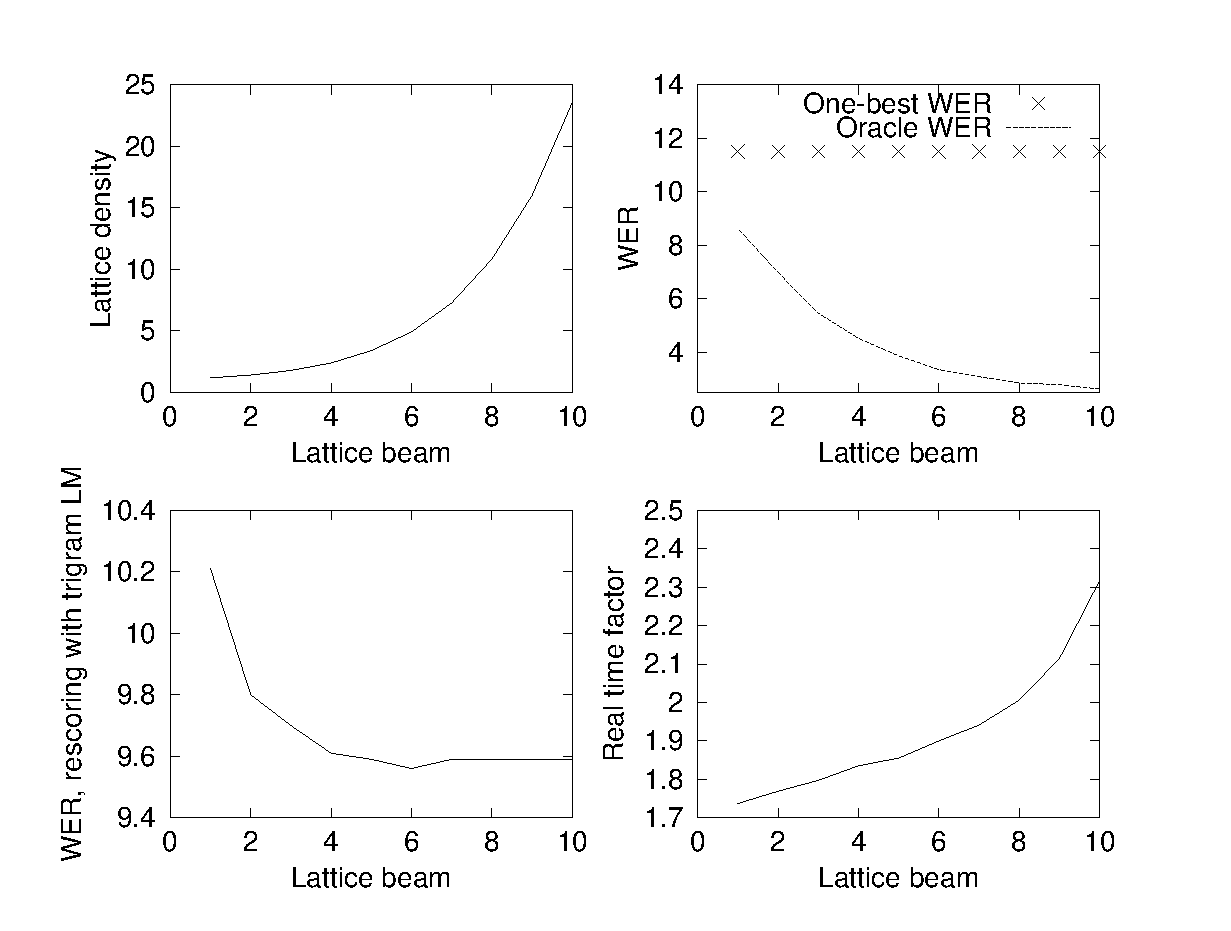
\includegraphics[width=0.9\columnwidth]{figures/latbeam.eps} 
 \vspace*{-0.1in}
 
   \caption{ { Lattice properties, varying lattice beam $\alpha$ (Viterbi pruning beam fixed at 15)} }
  \vspace{-0.15in}
  \label{fig:latbeam}
\end{figure}

Figure~\ref{fig:latbeam} shows how the lattice properties change as we vary
$\alpha$, with the Viterbi beam fixed at 15; Figure~\ref{fig:viterbibeam} varies
the Viterbi decoding beam, leaving $\alpha$ fixed at 7.  Lattice density is
defined as the average number of arcs crossing each frame.  We get all the
improvement from LM rescoring by increasing $\alpha$ to 4, and time taken
increases rapidly when $\alpha > 8$, so we recommend roughly $4 < \alpha < 8$ for
LM rescoring purposes.  We do not display the real-time factor of the
non-lattice-generating decoder on this data (2.26xRT) as it was actually slower
than the lattice generating decoder; this is possibly due to the overhead of
reference counting.  Out of vocabularly words (OOVs) provide a floor on the
lattice oracle error rate: of 333 test utterances, 87 contained at least one OOV
word, yet only 93 sentences (6 more) had oracle errors with $\alpha=10$.


\begin{figure}[t]
\centering
   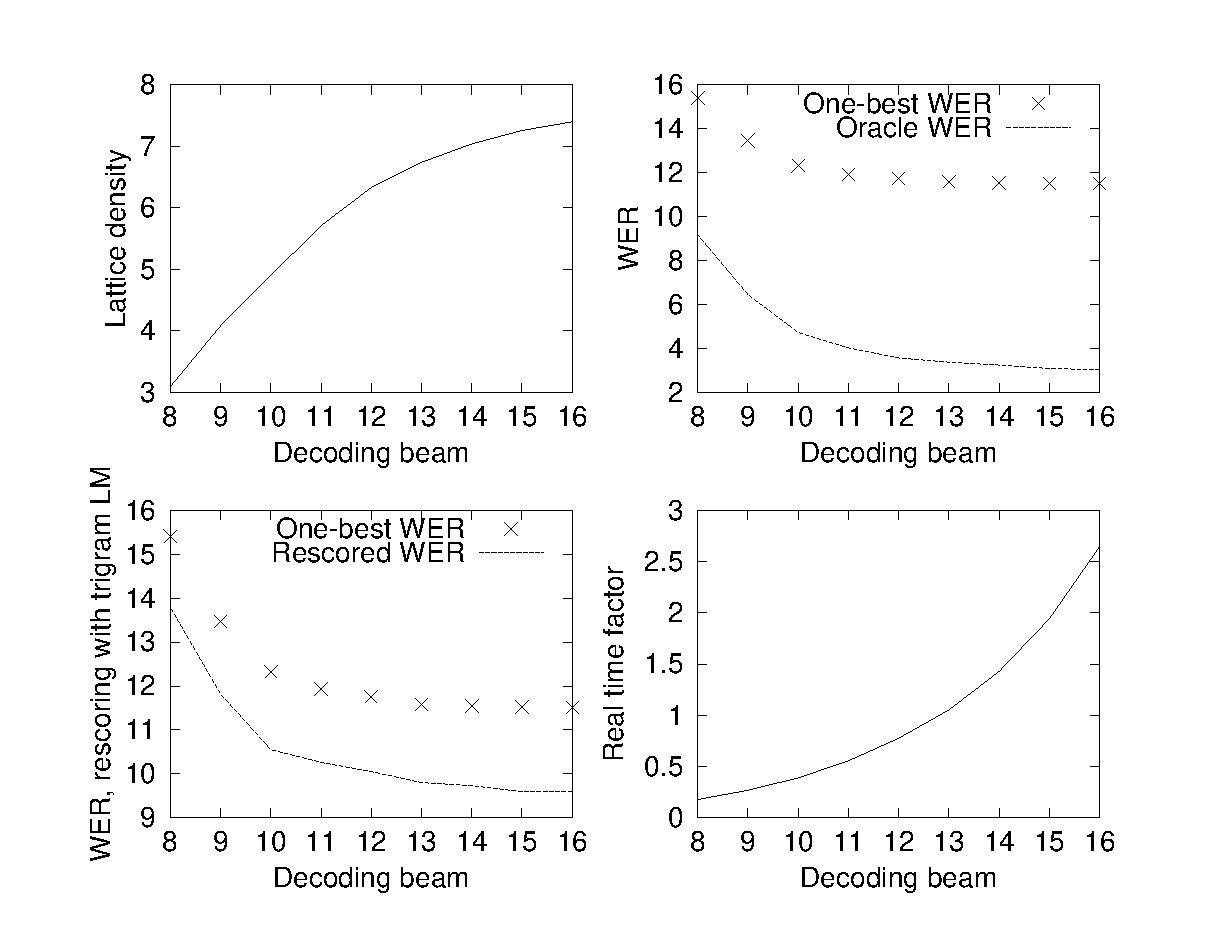
\includegraphics[width=0.9\columnwidth]{figures/decodebeam.eps} 
 \vspace*{-0.1in}
    \caption{ {Lattice properties, varying Viterbi pruning beam (lattice beam $\alpha$ fixed at 7)}}
  \label{fig:viterbibeam}
  \vspace{-0.15in}
\end{figure}


\vspace*{-0.1in}
\section{Conclusions}
\label{sec:conc}
\vspace*{-0.075in}

We have described a lattice generation method that is to our knowledge the first
efficient method that does not rely on the word-pair assumption of~\cite{ney_word_graph}.
It includes an ingenious way of obtaining HMM-state-level alignment information
via determinization in a specially designed semiring. 

\vspace*{-0.04in}
\footnotesize {
\vspace*{-0.1in}
\bibliographystyle{IEEEbib}
\bibliography{refs}
}

\end{document}


steps/decode_tri3a_latgen.sh
acwt=0.0625
beam=[15.0-7.0]
max_active=15000
lat_beam=[10.0-1.0]
max_arcs=50000 (75000 for lat_beam 10.0)
model=exp/tri3a/final.mdl
graph=exp/graph_tri3a_bg_left/HCLG.fst

scp=data/eval_nov92.scp

333 utterances
87 utterances contain OOV
42 utterances contain annotated noise (actually some more, but listed as OOV utterances here)

5641 tokens (some scripts count 5700 with 59 noise annotations)
107 OOV tokens
1.88% OOV token rate

253204 frames (2532 seconds)

19976 words in decoding vocabulary and LM (not counting <s>,</s>,<unk>)

average lattice link density per frame:
have a wide range over files: for example beam=15.0, lat_beam=9.0:
ranging from 1.5 to 167

running on blades, using 64bit version with double float and lattice-simple-decoder
realtime factor running on pcburget, 22989 frames (decode3.sh)

decoding with bigram LM:
decoding WER:      11.51%
ins/del/sub:       118/57/474   
utterances wrong:  227          

1) experiment: changing lattice beam:
(lattices 443c040w and 444c040i have been reduced from 10.0 to 8.1 because of determinization memory problems)

decoding beam:     15.0         15.0       15.0       15.0       15.0         15.0        15.0        15.0        15.0         15.0        15.0
lattice beam:      10.0          9.0        8.0        7.0        6.0          5.0         4.0         3.0         2.0          1.0         0.0
avg. link density: 23.56        16.0       10.82       7.26       4.91         3.38        2.38        1.77        1.4          1.17        1.0
realtime factor:    2.317        2.114      2.006      1.941     1.900         1.855       1.835       1.797       1.769        1.737       ---

oracle WER:         2.62%        2.78%      2.85%      3.08%      3.35%        3.86%       4.52%       5.46%       6.98%        8.62%      11.51%
ins/del/sub:       22/0/126     25/0/132   29/0/132   31/1/142   38/5/146     51/11/156   57/15/183   64/20/224   76/32/286    89/40/357   118/57/474
oracle utt wrong:  93           96         96         101        105          116         129         147         168          191         227

rescoring WER(15):  9.59%        9.59%      9.59%      9.59%      9.56%        9.59%       9.61%       9.70%       9.80%       10.21%      11.51%
ins/del/sub:       117/36/388                                    116/36/387   117/35/389  115/35/392  111/38/398  108/39/406   113/42/421  118/57/474
rescore utt wrong: 205                                           204          204         204         202         205          212         227

2) experiment: changing decoding beam:

decoding beam:     16.0        15.0          14.0          13.0         12.0         11.0         10.0          9.0 (1 utt partial) 8.0 (2 partial)
lattice beam:       7.0         7.0           7.0           7.0          7.0          7.0          7.0          7.0                7.0
avg. link density:  7.4         7.26          7.04          6.74         6.33         5.71         4.9          4.08               3.09
realtime factor:    2.646       1.941         1.428         1.052        0.775        0.555        0.388        0.267              0.177
decoding WER:      11.51%       11.51%       11.54%        11.58%       11.75%       11.93%       12.32%        13.47%             15.41%
ins/del/sub:       118/57/474   118/57/474   118/57/476    119/56/478   124/57/482   131/58/484   140/58/497    164/56/540         197/61/611
utterances wrong:  227          227          227           227          228          228          229           236                246

oracle WER:        3.03%        3.08%        3.24%         3.37%        3.56%        4.02%        4.72%         6.45%              9.18%
ins/del/sub:       30/1/140     31/1/142     35/2/146      38/2/150     42/3/156     54/6/167     55/7/204      73/13/278          118/22/378
oracle utt wrong:  100          101          105           108          112          119          128           153                184

rescoring WER(15): 9.59%        9.59%        9.73%         9.80%        10.05%       10.26%       10.55%        11.82% (1 failed)  13.79% (2 failed)
ins/del/sub:       116/36/389   117/36/388   115/37/397    117/38/398   123/39/405   132/39/408   141/37/417    ---                ---
rescore utt wrong: 205          205          206           206          207          209          208           220                235

3) bigram vs. trigram decoding:

decoding lm:       bigram       trigram,pruned  bigram        trigram,pruned   bigram (just to see whether wider beams still help)
decoding beam:     15.0         15.0            13.0          13.0             16.0 
lattice beam:       9.0          9.0             9.2           9.2             10.0 (already quite big for lattice-oracle - more than 6GB RAM used)
avg. link density: 16.0         14.98           14.86         13.58            24.84
rt factor(old):     3.17         3.26            1.75         1.77              4.54

decoding WER:      11.51%       10.57%          11.58%        10.80%           11.51%
ins/del/sub:       118/57/474   116/44/436      119/56/478    120/47/442       118/57/474
utterances wrong:  227          214             227           215              227

oracle WER:        2.78%        2.84%           3.05%         3.19%            2.61%
ins/del/sub:       25/0/132     30/0/130        30/2/140      33/1/146         21/0/126
oracle utt wrong:  96           96              103           107              92

rescoring WER(15):  9.59%       9.64%           9.80%         9.87%            9.59%
ins/del/sub:       117/36/388   115/34/395      117/38/398    119/38/400       116/36/389
rescore utt wrong: 205          205             206           209              205

4) lattice vs. n-best lists
decoding with trigram, pruned

decoding:          lattice      n-best         n-best/beam
decoding beam:     13.0         13.0           13.0  
lattice beam:      9.2          --             9.35 [6.0-12.5] (few outliers below/above)
N best:            --           <=20           206.96 [2-1600] (according to beam range and utterance)
max tokens:        15000        150k,700k      150000-770000
avg. link density: 13.58        14?            231.05
realtime factor:   1.77         12             crap

decoding WER:      10.80%       12.78% (why?)  14.96% (probably too low max tokens)
ins/del/sub:       120/47/442
utterances wrong:  215

oracle WER:        3.19%
ins/del/sub:       33/1/146
oracle utt wrong:  107

rescoring WER(15):  9.87%
ins/del/sub:       119/38/400
rescore utt wrong: 209

2.259 is baseline RT factor w/ decoding beam of 15, with simple-decoder.

note: paper# is 3887
passwd  CF8FECE1

